\section{Introduction}
\label{sec:intro} 
Estimation of hands and objects is fundamental and crucial for understanding meaningful interpretation of human action and
behavior. It provides enormous knowledge for environmental perception and teaching manipulating systems. With the advent of deep learning, pose estimation tasks have significantly made progress such as RGB-based \cite{cai20203d, zimmermann2017learning, gao2019variational, xiang2017posecnn, tremblay2018deep}, depth-based \cite{oberweger2017deepprior++, moon2018v2v, xiong2019a2j, ge20173d, cai2022ove6d, li2020category}, and RGB-D methods \cite{kazakos2018fusion, yuan20193d}. Jointly estimation of hands and objects under interaction, however, has attracted less attention due to chronic challenges. This requires simultaneously predicting the pose and shape of hands and objects during the hand manipulating the objects. In this paper, we propose a novel network to tackle this problem from RGB-D images. 

\begin{figure}[t]
\center
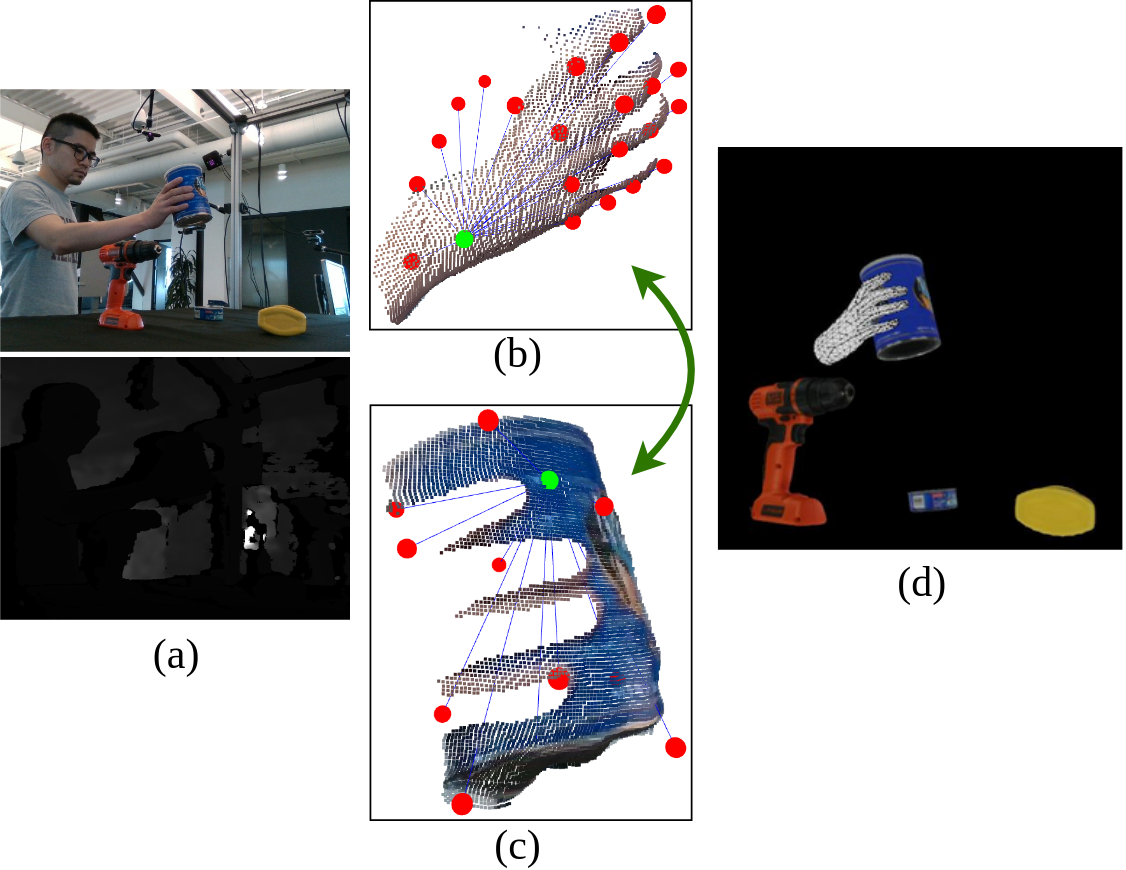
\includegraphics[width=\linewidth]{Figs/project_overview.png}
\label{fig:result_exp}
\caption{Our method captures features from both RGB and depth images (a) to vote for hand and object keypoints. (b) The hand point cloud and voting vectors (blue lines), each point on the hand (green point) votes for 21 MANO joints (red points). (c) The held object and voting vectors (blue lines), each point on the same object (green point) votes for $M=9$ selected keypoints (red points). The interaction relationships between the hand and the held object are learn by feeding voting vectors into a GCN. (d) The hand-object pose estimation result.}
\end{figure}

Joint hand-object pose estimation under interaction is a much more challenging problem. The hand shape is notorious for being self-occlusion. This problem is adversely serious in the context when the hand manipulating an object due to escalated occlusion. The naive approach is estimating the shape of the hands and objects seperately. Such methods leverage the success of object pose estimation and hand shape reconstruction independently without considering the correlations between themselves. They totally ignore the heavy interdependencies between hand pose on the held object's shape. Intuitively, the presence of object strongly defines and constrains the hand grasps and therefore limits the feasible hand gestures to a restricted number. Similarly, determining hand gestures provides a cue for estimating the shape and pose of the held object. Consequently, simultaneously predicting the shapes of both hand and object soonly catches the attention of computer vision researchers.  \cite{hasson2019learning, hasson2020leveraging, tekin2019h+, tse2022collaborative, liu2021semi, oikonomidis2011full, lu2021understanding, hasson2021towards, wang2020learning} joinly learn the hand and object poses from a single RGB image. Whereas, \cite{choi2017robust, zhang2021single, goudie20173d, oberweger2019generalized} focus on another input format, depth images, to achieve the expected results. However, they pose a threat to the prediction accuracy due to lack of the other type format input. With the prevalence of depth sensor, RGB-D image-based methods \cite{kyriazis2013physically, tsoli2018joint} appear to be a promising solution. Although numerous research has made an impressive success in a wide range of computer vision tasks. It still puzzles the reseacher community of how to effectively using RGB-D input for joint hand-object pose estimation.

In this paper, we propose a network termed adaptive fusion that extracts color and depth features and wisely combines them to generate the discriminative representation of input data. We embrace the fact that the favourable features conveyed by color and depth information differ across positions. At a specific pixel, the RGB feature may be much more compelling than the physical one but the other pixel may witness the opposite  situation. Our network learns to predict the weight factors that either amplifies the favourable features or inhibits the meaningless information. Therefore, it can thoroughly investiagte the meaningfulness and the beneficial contribution of RGB and Depth values at each position to effectively incorporate them together across all positions inspired by \cite{wang2019densefusion}. In other words, our proposal module does not solely integrate the geometric feature to the color one, but also tells to what extent the system should pay attention on each type of features at each position. 

To tackle the problem of adverse occlusion under the hand-object interaction contexts, we adopt the graph convolutional network (GCN) to introduce the interaction learning procedure that captures the correlations between hands and objects appearance. We firstly predict the hand and object keypoints by deep a Hough voting network. The network focuses on the keypoints of hands and objects instead of their centroids, which are dominant in detection and pose estimation tasks. This is because the centroid points are capable to represent the object's existence but cannot provide the information for hand-object interaction learning due to their properties of being away from the contacting surfaces and being virtual. The keypoints, hence, are favourable to GCN to absorb the geometric interdependencies and constraints between hand and object shapes. This facilitates our network can consider the shape-defining conditions that the hand puts on the manipulated object and in the reverse relation. Therefore, this boosts the pose estimation performance of our method when coping with the interaction contexts. We further conduct experiments on \textbf{dataset} to evaluate our method. Experimental results demonstrate that our approach performances significantly exceed the current state-of-the-art methods.

In brief, the main contributions of our work are:

\begin{itemize}
	\item We propose the adaptive fusion network to empower the capability of extracting features from RGB-D images. This network can learn both color and geometric features and then adaptively fuse them by either wisely and selectively magnifying the value features or weakening the useless one at each pixel. 
	 
	\item We introduce a GCN-based network to learn the interrelation between the hand and the manipulated object poses by examining their corresponding voting vectors. It allows to learn the hand pose under the impact of the object's existence and vice versa.
	 
	\item Experiments on benchmark datasets demonstrate that our approach can outweigh the state-of-the-art models for hand and object 3D pose estimation.
\end{itemize}



